
\section{Planificación}

\subsection{Iteraciones}

\textbf{Primera iteración} [3 semanas]
	\begin{enumerate} \itemsep -2pt
		\item Accediendo a la red pública de drones
		\item Recibiendo imágenes de los drones
		\item Procesando datos de bandas espectrales de las fotografías
		\item Interactuando con actuadores
	\end{enumerate}

\textbf{Segunda iteración} [2 semanas]
	\begin{enumerate} \itemsep -2pt
		\item Generando mediciones de estado del terreno / cultivos a partir de fotos procesadas
		\item Monitoreando el estado de salud de las plantas
		\item Obteniendo información del clima a partir de las micro-estaciones climatológicas del INTA.
		\item Calculando decisión según información recolectada y plan maestro
	\end{enumerate}

\textbf{Tercera iteración} [2 semanas]
	\begin{enumerate} \itemsep -2pt
		\item Iniciando seguimiento de cultivos / región
		\item Incorporando nuevas especies de cultivo (ABM Cultivo)
		\item Consultando planes maestros de cultivo provistos por el INTA / organismos privados (ABM Plan)
		\item Consultando estado de los cultivos
		\item Accediendo a la red privada de drones
	\end{enumerate}

\textbf{Cuarta iteración} [2 semanas]
	\begin{enumerate} \itemsep -2pt
		\item Supervisando acciones ordenadas a actuadores
		\item Agregando muestreo manual del estado de los cultivos / terreno
		\item Visualizando el mapa del estado del terreno
		\item Personalizando plan maestro de cultivo
		\item Agregando nuevos actuadores (ABM Actuador)
	\end{enumerate}

\textbf{Quinta iteración} [2 semanas]
	\begin{enumerate} \itemsep -2pt
		\item Logueando eventos del sistema
		\item Autenticando usuario (ABM Usuario)
		\item Autorizando usuario (ABMs Rol y Permiso)
		\item Revisando registro de eventos
	\end{enumerate}

\textbf{Sexta iteración} [2 semanas]
	\begin{enumerate} \itemsep -2pt
		\item Manejando fallas de servidores de INTA
		\item Descargando fotos offline de dron
		\item Organizando información almacenada entre nodos ArSat
		\item Encriptando / desencriptando información a almacenar
	\end{enumerate}

\subsection{Detalle Primera iteración}

\begin{itemize}
\item Identificación: E1
\item Tipo de iteración: Elaboración
\item Cantidad total de horas: 201.5h
\item Tareas:
	\begin{enumerate}
	\item Refinamiento de objetivos y requerimientos (2h)
	\item Análisis de riesgos (2h)
	\item Reconocimiento de casos de uso (3h)
	\item División de CU en iteraciones según prioridad (1h)
	\item Estimación de tiempos de CU (0.5h)
	\item Análisis de escenarios y atributos de calidad del sistema (2h)
	\item Diseño de arquitectura (8h)
	\item Realización de tareas de CU1 (50h)
	\item Realización de tareas de CU2 (40h)
	\item Realización de tareas de CU3 (63h)
	\item Realización de tareas de CU4 (30h)
	\end{enumerate}
\end{itemize}

\subsection{Plan de Proyecto}

\begin{figure}[h!]
  \centering
  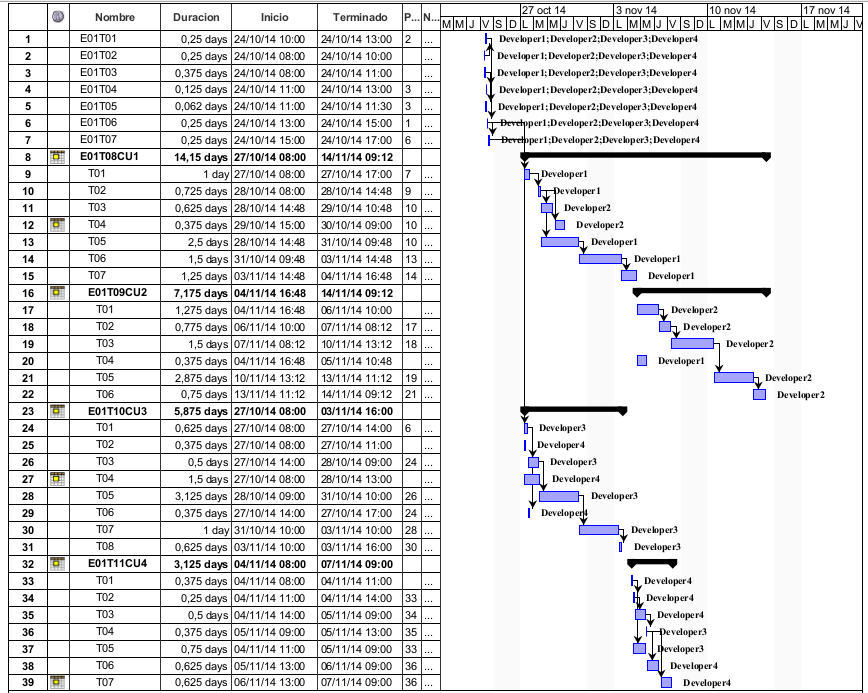
\includegraphics[width=1\textwidth]{plan.png}
  \caption{Diagrama Con las Iteraciones para la demo}
  \label{fig:clases4}
\end{figure}
